%%%% 导言区
%% 设定纸张大小为A4, 基本字体大小为12pt, 文章题目单独为一页, 
%% 文档类型为article
\documentclass[a4paper,12pt]{article}

%% en_preamble包含基本的宏包配置
%%%%%%%%------------------------------------------------------------------------
%%%% 日常所用宏包

%% 控制页边距
\usepackage[top=2cm, bottom=2cm, left=3.2cm, right=2.cm,includehead,includefoot]{geometry}

%% 控制项目列表
\usepackage{enumerate}

%% 多栏显示
\usepackage{multicol}

%% hyperref宏包,生成可定位点击的超链接,并且会生成pdf书签
\usepackage[%
    pdfstartview=FitH,%
    CJKbookmarks=true,%
    bookmarks=true,%
    bookmarksnumbered=true,%
    bookmarksopen=true,%
    colorlinks=true,%
    citecolor=blue,%
    linkcolor=blue,%
    anchorcolor=green,%
    urlcolor=blue%
]{hyperref}

%% 控制标题
\usepackage{titlesec}

%% 控制表格样式
\usepackage{booktabs}

%% 控制目录
\usepackage{titletoc}

%% 控制字体大小
\usepackage{type1cm}

%% 首行缩进,用\noindent取消某段缩进
\usepackage{indentfirst}

%% 支持彩色文本、底色、文本框等
\usepackage{color,xcolor}

%% AMS LaTeX宏包
\usepackage{amsmath}

%% 一些特殊符号
% \usepackage{bbding}

%% 支持引用
% \usepackage{cite}

%% LaTeX一些特殊符号宏包
% \usepackage{latexsym}

%% 数学公式中的黑斜体
% \usepackage{bm}

%% 调整公式字体大小:\mathsmaller, \mathlarger
% \usepackage{relsize}

%% 生成索引
% \makeindex

%%%% 基本插图方法
%% 图形宏包
\usepackage{graphicx}

%% 多个图形并排,参加lnotes.pdf
\usepackage{subfig}

% \begin{figure}[htbp]               %% 控制插图位置
%   \setlength{\abovecaptionskip}{0pt}
%   \setlength{\belowcaptionskip}{10pt}
                                     %% 控制图形和上下文的距离
%   \centering                       %% 使图形居中显示
%   \includegraphics[width=0.8\textwidth]{CTeXLive2008.jpg}
                                     %% 控制图形显示宽度为0.8\textwidth
%   \caption{CTeXLive2008安装过程} \label{fig:CTeXLive2008}
                                     %% 图形题目和交叉引用标签
% \end{figure}
%%%% 基本插图方法结束

%%%% pgf/tikz绘图宏包设置
\usepackage{pgf,tikz}
\usetikzlibrary{shapes,automata,snakes,backgrounds,arrows}
\usetikzlibrary{mindmap}
%% 可以直接在latex文档中使用graphviz/dot语言,
%% 也可以用dot2tex工具将dot文件转换成tex文件再include进来
%% \usepackage[shell,pgf,outputdir={docgraphs/}]{dot2texi}
%%%% pgf/tikz设置结束


%%%% fancyhdr设置页眉页脚
%% 页眉页脚宏包
\usepackage{fancyhdr}

%% 页眉页脚风格
\pagestyle{plain}

%% 有时会出现\headheight too small的warning
\setlength{\headheight}{15pt}

%% 清空当前页眉页脚的默认设置
%\fancyhf{}
%%%% fancyhdr设置结束


%%%% 设置listings宏包用来粘贴源代码
%% 方便粘贴源代码,部分代码高亮功能
\usepackage{listings}

%% 所要粘贴代码的编程语言
\lstloadlanguages{}

%% 设置listings宏包的一些全局样式
%% 参考http://hi.baidu.com/shawpinlee/blog/item/9ec431cbae28e41cbe09e6e4.html
\lstset{
showstringspaces=false,              %% 设定是否显示代码之间的空格符号
numbers=left,                        %% 在左边显示行号
numberstyle=\tiny,                   %% 设定行号字体的大小
basicstyle=\footnotesize,                    %% 设定字体大小\tiny, \small, \Large等等
keywordstyle=\color{blue!70}, commentstyle=\color{red!50!green!50!blue!50},
                                     %% 关键字高亮
frame=shadowbox,                     %% 给代码加框
rulesepcolor=\color{red!20!green!20!blue!20},
escapechar=`,                        %% 中文逃逸字符,用于中英混排
xleftmargin=2em,xrightmargin=2em, aboveskip=1em,
breaklines,                          %% 这条命令可以让LaTeX自动将长的代码行换行排版
extendedchars=false                  %% 这一条命令可以解决代码跨页时,章节标题,页眉等汉字不显示的问题
}
%%%% listings宏包设置结束


%%%% 附录设置
\usepackage[title,titletoc,header]{appendix}
%%%% 附录设置结束


%%%% 日常宏包设置结束
%%%%%%%%------------------------------------------------------------------------

%%%%%%%%------------------------------------------------------------------------
%%%% 英文字体设置结束
%% 这里可以加入自己的英文字体设置
%%%%%%%%------------------------------------------------------------------------

%%%%%%%%------------------------------------------------------------------------
%%%% 设置常用字体字号,与MS Word相对应

%% 一号, 1.4倍行距
\newcommand{\yihao}{\fontsize{26pt}{36pt}\selectfont}
%% 二号, 1.25倍行距
\newcommand{\erhao}{\fontsize{22pt}{28pt}\selectfont}
%% 小二, 单倍行距
\newcommand{\xiaoer}{\fontsize{18pt}{18pt}\selectfont}
%% 三号, 1.5倍行距
\newcommand{\sanhao}{\fontsize{16pt}{24pt}\selectfont}
%% 小三, 1.5倍行距
\newcommand{\xiaosan}{\fontsize{15pt}{22pt}\selectfont}
%% 四号, 1.5倍行距
\newcommand{\sihao}{\fontsize{14pt}{21pt}\selectfont}
%% 半四, 1.5倍行距
\newcommand{\bansi}{\fontsize{13pt}{19.5pt}\selectfont}
%% 小四, 1.5倍行距
\newcommand{\xiaosi}{\fontsize{12pt}{18pt}\selectfont}
%% 大五, 单倍行距
\newcommand{\dawu}{\fontsize{11pt}{11pt}\selectfont}
%% 五号, 单倍行距
\newcommand{\wuhao}{\fontsize{10.5pt}{10.5pt}\selectfont}
%%%%%%%%------------------------------------------------------------------------


%%%%%%%%------------------------------------------------------------------------
%%%% 一些个性设置

%% 设定页码方式,包括arabic、roman等方式
%% \pagenumbering{arabic}

%% 有时LaTeX无从断行,产生overfull的错误,这条命令降低LaTeX断行标准
%% \sloppy

%% 设定目录显示深度\tableofcontents
%% \setcounter{tocdepth}{2}
%% 设定\listoftables显示深度
%% \setcounter{lotdepth}{2}
%% 设定\listoffigures显示深度
%% \setcounter{lofdepth}{2}

%% 设定段间距
\setlength{\parskip}{0.3\baselineskip}

%% 设定行距
\linespread{1}

%% 中文破折号,据说来自清华模板
\newcommand{\pozhehao}{\kern0.3ex\rule[0.8ex]{2em}{0.1ex}\kern0.3ex}

%% 设定itemize环境item的符号
\renewcommand{\labelitemi}{$\bullet$}

%% 设定正文字体大小
% \renewcommand{\normalsize}{\sihao}

%%%% 个性设置结束
%%%%%%%%------------------------------------------------------------------------


%%%%%%%%------------------------------------------------------------------------
%%%% bibtex设置

%% 设定参考文献显示风格
\bibliographystyle{unsrt}

%%%% bibtex设置结束
%%%%%%%%------------------------------------------------------------------------


%% 如果不写中文的话就不需要引用xecjk_preamble里面的配置
%%%%%%%%------------------------------------------------------------------------
%%%% xeCJK相关宏包

\usepackage{xltxtra,fontspec,xunicode}

%% \CJKsetecglue{\hskip 0.15em plus 0.05em minus 0.05em}
%% slanfont: 允许斜体
%% boldfont: 允许粗体
%% CJKnormalspaces: 仅忽略汉字之间的空白,但保留中英文之间的空白。 
%% CJKchecksingle: 避免单个汉字单独占一行。
\usepackage[slantfont, boldfont]{xeCJK} 

%% 针对中文进行断行
\XeTeXlinebreaklocale "zh"             

%% 给予TeX断行一定自由度
\XeTeXlinebreakskip = 0pt plus 1pt minus 0.1pt

%%%% xeCJK设置结束                                       
%%%%%%%%------------------------------------------------------------------------

%%%%%%%%------------------------------------------------------------------------
%%%% xeCJK字体设置

%% 设置中文标点样式,支持quanjiao、banjiao、kaiming等多种方式
\punctstyle{kaiming}                                        
                                                     
%% 设置缺省中文字体
\setCJKmainfont[BoldFont={simhei.ttf}, ItalicFont={simkai.ttf}]{simsun.ttc}   
%% 设置中文无衬线字体
\setCJKsansfont[BoldFont={simhei.ttf}]{simkai.ttf}  
%% 设置等宽字体
\setCJKmonofont{simhei.ttf}                            

%% 英文衬线字体
\setmainfont{DejaVu Serif}                                  
%% 英文等宽字体
\setmonofont{DejaVu Sans Mono}                              
%% 英文无衬线字体
\setsansfont{DejaVu Sans}                                   

%% 定义新字体
\setCJKfamilyfont{song}{simsun.ttc}                     
\setCJKfamilyfont{kai}{simkai.ttf}
\setCJKfamilyfont{hei}{simhei.ttf}
\setCJKfamilyfont{fangsong}{simfang.ttf}
%\setCJKfamilyfont{lisu}{LiSu}
%\setCJKfamilyfont{youyuan}{YouYuan}

%% 自定义宋体
\newcommand{\song}{\CJKfamily{song}}                       
%% 自定义楷体
\newcommand{\kai}{\CJKfamily{kai}}                         
%% 自定义黑体
\newcommand{\hei}{\CJKfamily{hei}}                         
%% 自定义仿宋体
\newcommand{\fangsong}{\CJKfamily{fangsong}}               
%% 自定义隶书
%\newcommand{\lisu}{\CJKfamily{lisu}}                       
%% 自定义幼圆
%\newcommand{\youyuan}{\CJKfamily{youyuan}}                 

%%%% xeCJK字体设置结束
%%%%%%%%------------------------------------------------------------------------

%%%%%%%%------------------------------------------------------------------------
%%%% 一些关于中文文档的重定义

%% 数学公式定理的重定义

\newtheorem{example}{例}                                   
\newtheorem{algorithm}{算法}
%% 按section编号
\newtheorem{theorem}{定理}[section]                         
\newtheorem{definition}{定义}
\newtheorem{axiom}{公理}
\newtheorem{property}{性质}
\newtheorem{proposition}{命题}
\newtheorem{lemma}{引理}
\newtheorem{corollary}{推论}
\newtheorem{remark}{注解}
\newtheorem{condition}{条件}
\newtheorem{conclusion}{结论}
\newtheorem{assumption}{假设}

%% 章节等名称重定义
\renewcommand{\contentsname}{目\hspace{1.5cm}录}     
\renewcommand{\abstractname}{摘要}
\renewcommand{\indexname}{索引}
\renewcommand{\listfigurename}{插图目录}
\renewcommand{\listtablename}{表格目录}
\renewcommand{\figurename}{图}
\renewcommand{\tablename}{表}
\renewcommand{\appendixname}{附录}
\renewcommand{\appendixpagename}{附录}
\renewcommand{\appendixtocname}{附录}
\renewcommand\refname{参考文献} 

%% 设置chapter、section与subsection的格式
\titleformat{\chapter}{\centering\huge}{第\thechapter{}章}{1em}{\textbf}
%\titleformat{\section}{\centering\sanhao}{\hei \biaotiNR\thesection}{1em}{\textbf}
%\titleformat{\subsection}{\xiaosi}{\thesubsection}{1em}{\textbf}
%\titleformat{\subsubsection}{\xiaosi}{\thesubsubsection}{1em}{\textbf}

\usepackage{listings}

%%%% 中文重定义结束
%%%%%%%%------------------------------------------------------------------------


\title{浅谈机械零件可靠性设计}
\author{高星}
%\maketitle
\setcounter{secnumdepth}{5}

%%%% 导言区结束
%%%%%%%%------------------------------------------------------------------------

%%%%%%%%------------------------------------------------------------------------

%%%% 公共信息

%%%% 正文部分
\begin{document}
	
\begin{titlepage}
\begin{center}
%
\includegraphics[height=2.8cm]{images/hnsfdx} \vspace{1cm}
\mbox{}
\vspace{1cm}

{  \bf \kai \fontsize{36pt}{50pt}\selectfont \makebox[7em][s]{湖南师范大学}}
\vspace{0.5cm}

{  \bf \kai \fontsize{36pt}{50pt} \selectfont \makebox[7em][s]{工程与设计学院}}
\vspace{0.5cm}

\sihao 《机电一体化技术》课程考核 
\vfill
\vfill 

\sanhao \linespread{2}
 
 \makebox[3em][s]{姓名}:~
\underline{ \makebox[5cm]{高星}}\\
 \makebox[3em][s]{学号}:~
\underline{ \makebox[5cm]{201580180367}}\\ \makebox[3em][s]{教师}:~
\underline{ \makebox[5cm]{彭可}}\\			   
\vfill
%2017年2月20日
\end{center}
\end{titlepage}

\begin{titlepage}
\tableofcontents
\end{titlepage}

\sihao
\begin{center}
	 \erhao  \hei   数控转台控制系统设计 
\end{center} 
\sihao \setlength{\parindent}{2em}    

{\bf 摘 要: }
数控转台主要用于加工中心、数控镗床和铣床。本文对数控转台需求进行了分析,设计了数控转台机械部分的传动路线、主要部件参数的选择,对控制部分的步进电机进行了选择,解决了数控转台的工作原理和机械及控制的设计与计算。

{\bf 关键词: }机床附件;数控转台;齿轮;蜗轮蜗杆;步进电机;

\setcounter{section}{-1}
\section{引言} 
\sihao \setlength{ \baselineskip }{25pt}

数控转台主要用于加工中心、数控镗床和铣床,为加工中心和数控铣床提供了回转坐标,通过第四轴、第五轴驱动转台或分度头完成等分、不等分或连续的回转加工,完成复杂曲面加工,使机床原有的加工范围得以扩大。

传统的数控转台采用高精度蜗杆蜗轮等传动;
它的驱动是伺服系统的驱动方式。它可以与其他伺服进给轴联动。
它的进给、分度转位和定位锁紧都是由给定的指令进行控制的。转台的运动是由伺服电动机,经齿轮减速后由蜗杆传给蜗轮。

当转台静止时必须处于锁紧状态。

回转转台的导轨面由大型滚动轴承支承,并由深沟球轴承及双列向心圆柱滚子轴承保持准确的回转中心。数控转台的定位精度主要取决于蜗杆副的传动精度,因而必须采用高精度蜗杆副。在半闭环控制系统中,可以在实际测量转台静态定位误差之后,确定需要补偿角度的位置和补偿的值,记忆在补偿回路中,由数控装置进行误差补偿。在全闭环控制系统中,由高精度的圆光栅发出转台精确到位信号,反馈给数控装置进行控制。

回转转台设有零点,当它作回转运动时,先用挡铁压下限位开关,使转台降速,然后由圆光栅或编码器发出零位信号,使转台准确地停在零位。数控转台可以作任意角度的回转和分度,也可以作连续回转进给运动。

\section{需求分析}
数控转台是一种重要的机床附件,主要应用在加工中心和数控镗铣床上,俗称 “四轴” 。数控转台的应用,为机床提供了回转坐标,通过第四轴、第五轴驱动转台 完成等分、不等分或连续的回转加工,使客户加工复杂曲面变成可能,扩大了机床 的加工范围。近年来,随着国产数控机床向高速、高效、高精、柔性化、环保方面 迅猛发展,用户对零件加工的
要求也越来越高,加工中心(特别是四轴、五轴)的 需求也在增加,与之相应的数控转台的需求也随之发展。

国内的数控转台市场主要被我国内地和台湾地区的生产厂家所占领,少量高端 产品由日本、德国、美国等公司占领,国内产品主要以中低档产品为主。 内地最具竞争力的生产厂家是烟台环球机床附件集团有限公司, 产品体系完善, 规格种类齐全,设计开发和制造经验丰富。台湾的生产厂家比如德川机械股份有限 公司是专业数控转台制造商之一。国外的专业生产厂家有日本的 NIKKEN(日研) 、 德国 Peiseler 美国 HASS 公司等。国内的数控转台产品与国外产品相比仍有一定差 距,主要表现在数控转台的速度、精度、可靠性上。通过优化蜗轮副的材料和制造 工艺、端齿盘的材料和制造工艺、装配工艺以及其它技术手段,可以提高国内产品 的总体质量。国内产品虽然在地域上具有维修方便快捷的优势,但是提高转台的可 靠性和耐用度仍是将来努力的重点。

我国的功能部件发展已经跟不上机床行业发展的步伐,成为民族机床工业发展 的瓶颈。国家规划中,对功能部件的发展予以了大力的支持,数控转台 的开发研制和技术创新得到了发展的契机。数控转台的发展趋势是:在规格上向两 头延伸,即开发小型和大型转台;在性能上将研制新结构,采用新材料,大幅度提 高工作台转速和转台的承载能力;在形式上研制两轴联动和多轴并联回转的数控转 台。国内厂家要加快自主创新,广泛应用新技术、新材料,瞄准国际先进水平,尽 快缩短与国外先进水平的差距,走专业化、产业化、社会协作化的路子,形成规格 齐全、 性能优越、 形式多样的中高档次数控转台产品生产模式, 在产品质量、 性能、 结构创新、精度稳定性、品牌信誉、外观造型等方面有所突破,做大做强中国数控 转台产业。

\section{机械部分设计}

\subsection{传动方案的选择}
\subsubsection{传动方案传动时应满足的要求}
数控转台一般由原动机、传动装置和转台组成,传动装置在原动机和转台之间传递运动和动力,并可实现分度运动。在本课题中,原动机采用应采用步进电机,转台为T形槽转台,传动装置由齿轮传动和蜗杆传动组成。

合理的传动方案主要满足以下要求:
\begin{enumerate}
	\item 机械的功能要求:应满足转台的功率、转速和运动形式的要求。
	\item 工作条件的要求:例如工作环境、场地、工作制度等。
	\item 工作性能要求:保证工作可靠、传动效率高等。
	\item 结构工艺性要求;如结构简单、尺寸紧凑、使用维护便利、工艺性和经济合理等。
\end{enumerate}
\subsubsection{传动方案及其分析}
由图\ref{方案设计}所示,数控转台的传动方案有两种:方案一为一级和二级都是齿轮传动;方案二为一级齿轮传动,二级蜗杆传动。

	\begin{figure}[htb]
		\begin{center}
			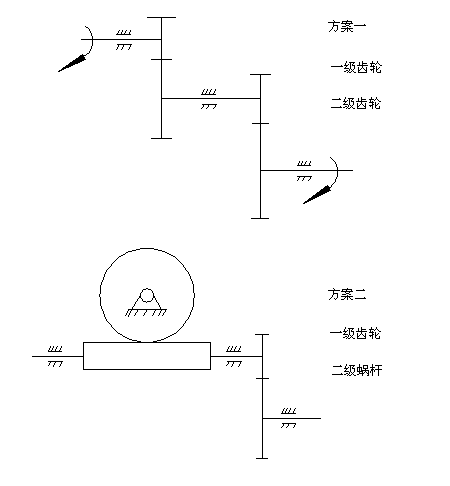
\includegraphics[width=9cm]{images/1}
		\caption{方案设计}  \label{方案设计}
	\end{center}
	\end{figure}

方案一的最大缺陷是:
\begin{enumerate}
	\item 总传动比小;
\item 占用空间大;
\item 只能使转台完成回转功能,无法使转台完成自锁。

\end{enumerate}

而方案二虽然传动效率低,但以上三个功能全部都能完成自锁。

所以数控转台传动方案为方案二:步进电机——齿轮传动——蜗杆传动——转台。

该传动方案分析如下:
\\
齿轮传动承受载能力较高 ,传递运动准确、平稳,传递 功率和圆周速度范围很大,传动效率高,结构紧凑。

蜗杆传动有以下特点:
\begin{enumerate}
	\item 传动比大,在分度机构中可达1000以上。与其他传动形式相比,传动比相同时,机构尺寸小,因而结构紧凑。
\item 传动平稳 蜗杆齿是连续的螺旋齿,与蜗轮的啮合是连续的,因此,传动平稳,噪声低。
\item 可以自锁 当蜗杆的导程角小于齿轮间的当量摩擦角时,若蜗杆为主动件,机构将自锁。这种蜗杆传动常用于起重装置中。
\item 效率低、制造成本较高  蜗杆传动方面:齿面上具有较大的滑动速度,摩擦磨损大,故效率约为0.7-0.8,具有自锁的蜗杆传动效率仅为0.4左右。为了提高减摩擦性和耐磨性,蜗轮通常采用价格较贵的有色金属制造。

\end{enumerate}

由以上分析可得:将齿轮传动放在传动系统的高速级,蜗杆传动放在传动系统的低速级,传动方案较合理。


\subsection{齿轮传动的设计}
如图\ref{一级齿轮传动}所示,一级传动为齿轮传动,其中1为小齿轮,2为大齿轮,传动比为3。
	\begin{figure}[htb]
	\begin{center} 
		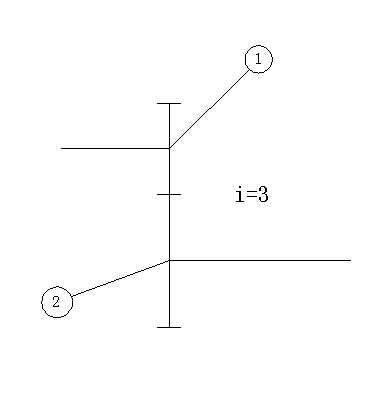
\includegraphics[width=4cm]{images/2}
		\caption{一级齿轮传动}  \label{一级齿轮传动}
	\end{center}
\end{figure}

\subsubsection{选择齿轮传动的类型与材料}
\begin{enumerate}
\item 选用直齿圆柱齿轮传动;
\item 选用7级精度;
\item 选择小齿轮材料为40Gr(调质),硬度为280HBS,大齿轮材料为45钢(调质);
\item 选小齿轮齿数Z=24,大齿轮齿数取Z=72
\end{enumerate}

\subsubsection{按齿面强度设计}
$$  d_1t \geq 2.32\sqrt[3]{\frac{KT_1}{\phi d} \bullet \frac{u\pm 1}{u} \bullet \left( \frac{Z_e}{[\sigma _H]}   \right)^2} $$
\paragraph{确定公式内的各计算数值}
\begin{enumerate}
	\item 试选载荷系数$K_t=1.3$;
	\item 计算小齿轮传递的转矩  $$ T_1=\frac{95.5\times 10^5 P_1}{n_1}=1.81\times 10^4 N\bullet mm$$
	\item 查表得齿宽系数 $ \phi d=1$ ;
	\item 材料的弹性影响系数 $Z_E=189.9 MP_0^{\frac{1}{2}}$
	\item 按齿面硬度查的小齿轮的接触疲劳强度极限$\sigma _{H lim1}=600MP_a $;大齿轮的接触疲劳强度$\sigma _{H lim2}=550MP_a $
	\item 计算应力循环次数: $$N_1=30n_1jL_b=60\times 1980 \times (2\times 8\times 250\times 8)=3.8\times 10^9$$
	$$N_2=\frac{N_1}{3}=1.27\times 10^9$$
	\item 取接触疲劳寿命系数$K_{HN1}=0.90$; $K_{HN2}=0.95$;
	\item  计算接触疲劳许用应力,取失效概率为1\%,安全系数S=1
	 $$ [\sigma_H]_1= \frac{K_{HN1}\sigma_{lim1}}{S} =0.9\times 600=540MPa $$
	  $$ [\sigma_H]_2= \frac{K_{HN2}\sigma_{lim2}}{S} =0.9\times 550=522.5MPa $$
\end{enumerate}

\paragraph{计算}
\begin{enumerate}
\item 试算小齿轮的分度圆直径$d_{1t}$,代入$[\sigma _H]$中较小的值
$$d_u\geq 65.28mm$$
\item 计算周转速度$v$ $$v=\frac{\pi d_{1t}n_1}{60\times 1000}=6.76m/s$$ \item 计算齿宽$b$ $$ b=\phi d \bullet d_{1t}=65.28mm$$
\item 计算分度圆直径: $$ d_1= d_u \sqrt[3]{\frac{K}{K_t} }=70.8mm$$
\item 计算模数$m$ $$ m=\frac{d_1}{Z_1}=3.22$$
\end{enumerate}
	可取标准值$m=3mm$,小齿轮齿数取$Z_1=24$。
	
\subsubsection{几何尺寸计算}
	
\begin{enumerate}
	\item 计算分度圆直径 $$d_1=Z_1\bullet m=72mm$$ $$d_2=Z_2\bullet m=72mm$$
	\item 中心距 $$ a=\frac{d_1+d_2}{2} =144$$
	\item 计算齿轮宽度 $$b=\phi d d_1 =72mm$$
   取 $B_1=75mm$、$B_2=70mm$
\end{enumerate}

\subsubsection{结构设计}
如图\ref{小齿轮}、\ref{大齿轮}所示两齿轮均为实心结构的齿轮,齿轮与轴采用单键连接。
\begin{figure}[htb]
	\begin{center} 
		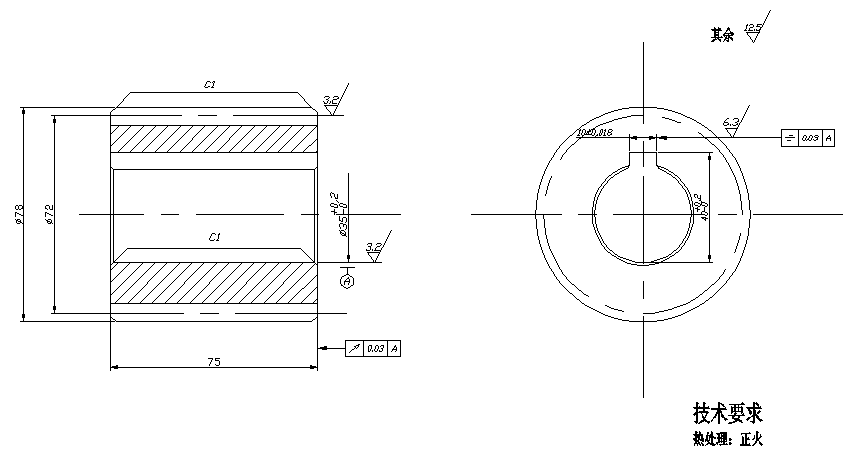
\includegraphics[width=0.7\textwidth]{images/3}
		\caption{小齿轮}  \label{小齿轮}
	\end{center}
\end{figure}
\begin{figure}[htb]
	\begin{center} 
		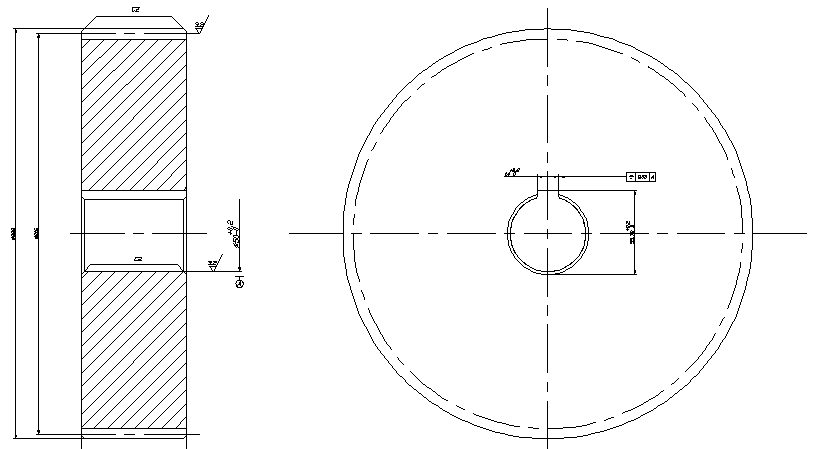
\includegraphics[width=0.7\textwidth]{images/4}
		\caption{大齿轮}  \label{大齿轮}
	\end{center}
\end{figure}

\subsection{蜗轮及蜗杆的选用与校核}
\subsubsection{选择蜗杆传动类型}
根据GB/T10085-1988的推荐,采用渐开线蜗杆(ZI)
\subsubsection{选择材料}
考虑到蜗杆传动功率不大,速度只是中等,故蜗杆用45钢;因希望效率高些,耐磨性好些,故蜗杆蜗杆螺旋齿面要求淬火,硬度为45-55HRC。蜗杆用铸锡磷青铜ZcuSn10P1,金属模铸造。为了节约贵重的有色金属,仅齿圈用青铜制造,而轮芯用灰铸铁HT100制造。
\subsubsection{按齿面强度进行设计}
根据闭式蜗杆传动的设计准则,传动中心距:
$$a\geq \sqrt[3]{KT_2\left( \frac{Z_EZ_p}{[\sigma _H]} \right)^2 }$$
\begin{enumerate}
	\item 确定作用在蜗杆上的转矩
	
	按$Z_1=2$,估取效率$ \eta =0.75$,则
	$$ T_2=9.55\times 10^6 \frac{P_2}{n_2} =9.55\times 10^6 \frac{p\eta }{n_2/i_{12}}=8247727 N\bullet mm$$
	\item 确定载荷系数
	
	因工作载荷较稳定,故取载荷分布不均匀系数$K_\beta=1$;选取使用系数$K_A=1.15$;由于载荷系数不高,冲击不大,可取动载荷系数$K_v=1.05$;则
$K=K_A K_\beta K_v=1.21$
	
	\item 确定弹性影响系数$Z_E$
	
	因选用的是铸锡磷青铜蜗轮和钢蜗杆相配,故$Z_E=160MP_a^\frac{1}{2}$。

\item 确定接触系数 $Z_p$
先假设蜗杆分度圆直径$d_1$和传动中心距$a$的比值$\frac{d_1}{a}=0.35$,得$Z_p=2.9$。

	\item 确定许用接触应力$[\sigma_H]$
	
	根据蜗轮材料为铸锡磷青铜ZcuSnP1,金属模铸造,蜗杆螺旋齿面硬度>45HRC,查得蜗轮的基本许用应力$[\sigma_H]=268MP_a$。
	
 	  应力循环次数    $N=60jn_2L_h=60\times 1 \times \frac{1980}{60}\times 8 \times 2 \times 250 \times 8 = 6.056\times 10^7$
 	  
 	  寿命系数 $K_{HN}=\sqrt[8]{\frac{10^7}{6.056\times 10^7}}=0.99$
	
	则 $[\sigma_H]=K_{HN}\bullet [\sigma_H]'=0.99\times 268 =266MPa$
	
	\item  计算中心距  $$a \geq \sqrt[3] {1.21\times 8247727 \times \left(\frac{160\times 2.9}{260} \right) ^2}=198mm$$
	
	取中心距$a=200mm$,因$i=20$,
	取模数$m=8$,蜗杆分度圆直径$d_1=80mm$。
	这时$\frac{d_1}{a}=\frac{80}{200}=0.4$,
   得接触系数$Z_p'=2.74$,
	因为$Z_p'<Z_p$,因此以上计算结果可用。
\end{enumerate}

\subsubsection{蜗杆与蜗轮的主要尺寸与参数}
\begin{enumerate}
	\item 蜗杆
	
	轴向齿距$P_a=25.133mm$;\\直径系数$q=10$;\\齿顶圆直径$d_{a1}=96mm$;\\齿根圆直径$d_{f1}=60.8mm$;\\分度圆导程角$\gamma=11\textdegree 18' 36"$;\\蜗杆轴向齿厚$S_a=12.5664mm$。
	
	\item 蜗轮
	
	蜗轮齿数$Z_2=41$;变位系数$x_2=-0.5$;\\
	验算传动比$i=\dfrac{Z_2}{Z_1}=\dfrac{41}{2}=20.5$,这时传动比误差为$\dfrac{20.5-20}{20}=2.5\%$,是允许的。\\
	蜗轮分度圆直径$d_2=mZ_2=8\times 41=328mm$。\\
	蜗轮喉圆直径$d_{a2}=d2+2h_{a2}=344mm$。\\
	蜗轮齿根圆直径$d_{f2}=d_2-2h_{f2}=308.8mm$。\\
	蜗轮咽喉圆半径$r_{g2}=a-\dfrac{1}{2}d_{a2}=28mm$。
	
\end{enumerate}

\section{控制部分电机的选择}
\subsection{步进电机的原理}
步进电机是一种能将数字输入脉冲转换成旋转或直线增量运动的电磁执行元件。每输入一个脉冲,电机转轴步进一个步距角增量。电机总的回转角与输入脉冲数成正比例,相应的转速取决于输入脉冲频率。 

步进电机是机电一体化产品中关键部件之一,通常被用作定位控制和定速控制。步进电机惯量低、定位精度高、无累积误差、控制简单等特点。广泛应用于机电一体化产品中,如:数控机床、包装机械、计算机外围设备、复印机、传真机等。
 
选择步进电机时,首先要保证步进电机的输出功率大于负载所需的功率。而在选用功率步进电机时,首先要计算机械系统的负载转矩,电机的矩频特性能满足机械负载并有一定的余量保证其运行可靠。在实际工作过程中,各种频率下的负载力矩必须在矩频特性曲线的范围内。一般地说最大静力矩大的电机,负载力矩大。 

选择步进电机时,应使步距角和机械系统匹配,这样可以得到机床所需的脉冲当量。在机械传动过程中为了使得有更小的脉冲当量,一是可以改变丝杆的导程,二是可以通过步进电机的细分驱动来完成。但细分只能改变其分辨率,不改变其精度。精度是由电机的固有特性所决定。 

选择功率步进电机时,应当估算机械负载的负载惯量和机床要求的启动频率,使之与步进电机的惯性频率特性相匹配还有一定的余量,使之最高速连续工作频率能满足机床快速移动的需要。
\subsection{步进电机的选择及运动参数的计算}
许多机械加工需要微量进给。要实现微量进给,步进电机、直流伺服交流伺服电机都可作为驱动元件。步进电机的特点:一是过载性好。其转速不受负载大小的影响,不像普通电机,当负载加大时就会出现速度下降的情况,所以步进电机使用在对速度和位置都有严格要求的场合;二是控制方便。步进电机是以“步”为单位旋转的,数字特征比较明显,这样就给计算机控制带来了很大的方便,反过来,计算机的出现也为步进电机开辟了更为广阔的使用市场;三是整机结构简单。传统的机械速度和位置控制结构比较复杂,调整困难,使用步进电机后,使得整机的结构变得简单和紧凑。所以选择步进电机的计算如下:

\subsubsection{电机的选择}
按照工作要求和条件选两相混合式步进电机
\subsubsection{功率}
工作所需功率为: $$ P_w = F_w V_w/1000\eta^wkW$$
$$P_w=T_{nw}/9950\eta^wkW$$
式中$T=150N\times M$,$\eta_w=36 r/min$ 电机工作效率,$\eta_w=0.97$ 
 $$Pw=150\times 36/(9950\times 0.97 )=3.9kw$$
电机所需的输出功率为:
$$P_o=P_w/\eta$$
则取电机额定功率为:$P_w=3.8$。
\subsubsection{转矩}
由齿轮的转矩可得:$$ T=\dfrac{95.5\times 10^5 p}{n} =1.81 \times 10^4 N\bullet mm$$
\subsubsection{确定电机转速}
取:
齿轮传动比:3-5,

蜗杆传动比:15-32,

则总的传动范围为:
$i=i_1\times i_2 =3\times 15-5*32 =45-160$

电机转速的范围为
 $N=i\times n_m = (45\sim 160)\times 36=1620\sim 5760 r/min$
为降低电机的重量和价格,选取常用两相混合式步进电机 11BYG250D-0502。

\subsubsection{利用步距角检验}
主要技术参数中,回转精度:$0.03°$、$i=60 $ 可得步距角为: $$\alpha=0.03°\times i=1.8°$$
计算的值与11BYG250D-0502步进电机的步距角相吻合。11BYG250D-0502步进电机满足条件。

\section{结束语}

通过传动方案的设计,机械部分的设计和控制系统的设计,以及相关元件的正确选择和参数的正确计算,本书库转台理论上能够达到所要求的相关功能,在硬件和软件都良好和正常的情况下,此数控分度转台能较好地完成相应的操作。本文设计的数控转台,仅有一个自由度。若在此基础上增加一个或多个自由度,那么工作台的应用范围将会更广,目前市场上多自由度的工作台需求量很大。所以若设计多自由度的数控转台,将会很有价值。

\vspace{4em}

{ \noindent \sanhao \bf 参考文献:}
\begin{enumerate}[{[1]}]
	\item 崔旭芳.数控回转转台的原理和设计[J].技术交流,2008,(3):23-27
	
	\item 顾华锋.数控机床回转转台动态性能分析与仿真[J]. 机床与液压,2008,(36):216-220
	
	\item 王友林.数控双转轴式回转转台的结构与工作原理[J]. 煤矿机械,2009,(30):102-103 
	
	\item 张立莹.回转数控转台夹紧机械浅析[J]. 制造技术,2001,(3):102-103 
	
	\item  李智强.基于CAN总线的高精度小型数控转台示教与设计[J].功能部件,2008,(6)158-16
 
	
	\item 何雪明.数控技术[M].武汉:华中科技大学出版社,2006.9
 
	
	\item  钟雯.机械类毕业设计选题精选[M].北京:化学工业出版社,2010.1 
	
	\item 杨萍.数控转台设计[J].组合机床自动化加工技术,1996,(8):18-42 
	
	\item 刘国庆,孙国民.齿轮泵的异常噪声问题[J].工程机械.1997(9) 
\end{enumerate}



%%中文习惯是设定首行缩进为2em。注意此设置一定要在document环境之中,这可能与\setlength作用范围相关
%\setlength{\parindent}{2em}
%
%\title{XecjkTemplateTest}
%\author{XiaoHanyu}
%\maketitle
%
%\tableofcontents
%\listoffigures
%%\listoftablescontent
%
%\section{基本文字测试}
\label{sec:1}
我叫肖晗宇,来自浙江大学计算机学院,热爱开源软件、旅行、摄影,推崇互助共享的精神理念。

My name is Xiao Hanyu, a student from Computer Science and Technology of Zhejiang University, I love open source software, travelling all over the world, photography, and so on. 

我喜欢\LaTeXe,也推荐大家来学习使用\LaTeXe,以下是比较不错的学习资源:

\begin{enumerate}
\item LaTeX companion
\item The TeXbook
\end{enumerate}


\section{图形图像测试}
\subsection{插图测试}
Hand in Hand:\ref{fig:hand_in_hand}
\begin{figure}[htbp]
\centerline{\includegraphics[width=0.6\textwidth]{images/hand_in_hand.png}}
\caption[]{\label{fig:hand_in_hand} 手拉手}
\end{figure}

\subsection{pgf/tikz绘图测试}
图\ref{fig:monotonic_chain}是用pgf/tikz宏包作的图形,用以说明计算几何相关定理。

\begin{figure}
\centering
\begin{tikzpicture}[line width=2pt]
\draw (-1,0) -- (8,0);
\draw (0,-1) -- (0,8);
\draw[step=.5cm, very thin] (0,0) grid (7.2,7.2);

\coordinate [label=above:$A$] (A) at (1, 4);
\coordinate [label=left:$B$] (B) at (0.5, 3.5);
\coordinate [label=left:$C$] (C) at (1, 3);
\coordinate [label=left:$D$] (D) at (0.3, 1.3);
\coordinate [label=below:$E$] (E) at (1, 1);

\draw[blue] (A) -- (B) -- (C)  -- (D) -- (E);
\draw[blue] (2, 0) -- (2, 6);

\coordinate [label=right:$A'$] (A') at (2, 4);
\coordinate [label=right:$B'$] (B') at (2, 3.5);
\coordinate [label=right:$C'$] (C') at (2, 3);
\coordinate [label=right:$D'$] (D') at (2, 1.3);
\coordinate [label=right:$E'$] (E') at (2, 1);

\draw[blue] (A) -- (A');
\draw[blue] (B) -- (B');
\draw[blue] (C) -- (C');
\draw[blue] (D) -- (D');
\draw[blue] (E) -- (E');

\coordinate [label=above:$a$] (a) at (5, 4);
\coordinate [label=left:$b$] (b) at (4.5, 4.5);
\coordinate [label=left:$c$] (c) at (5, 3);
\coordinate [label=left:$d$] (d) at (4.3, 1.3);
\coordinate [label=below:$e$] (e) at (5, 1.3);

\draw[green] (a) -- (b) -- (c)  -- (d) -- (e);
\draw[green] (6, 0) -- (6, 6);

\coordinate [label=right:$a'$] (a') at (6, 4);
\coordinate [label=right:$b'$] (b') at (6, 4.5);
\coordinate [label=right:$c'$] (c') at (6, 3);
\coordinate [label=right:$d'$] (d') at (6, 1.3);
\coordinate [label=right:$e'$] (e') at (6, 1.3);

\draw[green] (a) -- (a');
\draw[green] (b) -- (b');
\draw[green] (c) -- (c');
\draw[green] (d) -- (d');
\draw[green] (e) -- (e');
\end{tikzpicture}
\caption{Monotonic polygonal chains}
\label{fig:monotonic_chain}
\end{figure}

\section{表格测试}
\begin{table}[htbp]
  \centering
  \begin{tabular}[htbp]{r|l}
    \toprule
    日期 & 任务 \\
    \midrule
    2011.5 & 完善此份文档 \\
    2011.6 & 完善安装脚本 \\
    \bottomrule
  \end{tabular}
  \caption{表格}
  \label{tab:table1}
\end{table}

\section{源代码高亮测试}

以下是\href{http://acm.zju.edu.cn/onlinejudge/showProblem.do?problemCode=1372}{ZOJ 1372}的解题c++代码:

\begin{lstlisting}[language=c++]
#include <iostream>
#include <string>
using namespace std;
 
const long max_points = 100;
const long infinity = 1000001;
 
int p, r, length, g[max_points][max_points];
bool flag;
 
class vertex
{
public:
    int distance;
    bool visited;
};
 
vertex v[max_points];
 
void initial()
{
    for(int i = 1; i <= p; i++)
        for(int j = 1; j <= p; j++)
            g[i][j] = infinity;
}
 
void prim(int origin)
{
    int temp_min;
    int temp_v = 0;
    int sum = 0;
 
    for(int i = 1; i <= p; i++)
    {
        v[i].distance = g[i][origin];
        v[i].visited = false;
    }
 
    v[origin].distance = 0;
    v[origin].visited = true;
 
    sum++;
 
    while (sum < p)
    {
        temp_min = infinity;
        for(int i = 1; i <= p; i++)
            if(v[i].visited == false && v[i].distance < temp_min)
            {
                temp_min = v[i].distance;
                temp_v = i;
            }
         
        if(temp_min < infinity)
        {
            length += v[temp_v].distance;
            v[temp_v].visited = true;
            sum++;
        }
        else
        {
            flag = true;
            break;
        }
 
        for(int i = 1; i <= p; i++)
        {
            if(v[i].visited == false && v[i].distance > g[i][temp_v])
            {
                v[i].distance = g[i][temp_v];
            }
        }
    }
}
 
int main(int argc, char *argv[])
{
    int a, b, c;
 
    while(cin >> p)
    {
        if(p == 0)
            break;
        cin >> r;
 
        initial();
 
        for(int i = 0; i < r; i++)
        {
            cin >> a >> b >> c;
            if(c < g[a][b])
                g[a][b] = g[b][a] = c;
        }
        length = 0;
        prim(1);
 
        cout << length << endl;
    }
 
    return 0;
} 
\end{lstlisting}

\section{数学公式测试}

著名的爱因斯坦质能方程(\ref{eq:emc2}):

\begin{equation}
  \label{eq:emc2}
  E=mc^2
\end{equation}

计算$f(x)=x^2$的不定积分(\ref{eq:2}):

\begin{equation}
  \label{eq:2}
  \int x^2 dx = \frac{1}{3} x^3
\end{equation}
\section{参考文件测试}
参考文件最好使用bibtex,关于bibtex的使用方法,你可以自行查阅相关文献。

这里是参考文献\cite{c_minigui}

%%%%%%%%%------------------------------------------------------------------------
%%%% 附录

% \appendix    
% \appendixpage
%% 将附录条目添加到contents
% \addappheadtotoc

%%%% 附录结束
%%%%%%%%------------------------------------------------------------------------

%
%%%加入参考文献支持
%\bibliography{data/main}
%%%解决目录中没有相应的参考文献的条目问题
%\addcontentsline{toc}{section}{\refname}
\end{document}
%%%%正文部分结束
%%%%%%%%------------------------------------------------------------------------
